% ============================================================================
\section{Preliminaries}
\label{sec:preliminaries}
% ============================================================================

Let $G$ be a (not necessarily simple) \emph{topological graph}, that is, $G$ is a graph drawn on the plane, so that the vertices of $G$ are distinct points in the plane, its edges are Jordan courves joining the corresponding pairs of points, and:%
%
\begin{inparaenum}[(i)]
\item no edge passes through a vertex different from its endpoints, 
\item no edge crosses itself and 
\item no two edges meet tangentially.
\end{inparaenum}
Let $\Gamma(G)$ be such a drawing of $G$. The \emph{crossing graph} $\mathcal{X}(G)$ of $G$ has a vertex for each edge of~$G$, while two vertices of $\mathcal{X}(G)$ are connected by an edge if and only if the corresponding edges of $G$ cross in $\Gamma(G)$. A connected component of $\mathcal{X}(G)$ is called \emph{crossing component}. Observe that the set of crossing components of $\mathcal{X}(G)$ define a partition of the edges $G$. Given an edge $e$ of $G$ we denote by $\mathcal{X}(e)$ the crossing component of $\mathcal{X}(G)$ which contains $e$. 

An edge $e$ in $\Gamma(G)$ is called a \emph{topological edge} (or simply edge, if this is clear in the context). Edge $e$ is called \emph{true-planar}, if it is not crossed by any other edge in $\Gamma(G)$. The set of all true-planar edges of $\Gamma(G)$ forms the so-called \emph{true-planar skeleton} of $\Gamma(G)$, which we denote by $\Pi(G)$. Since $G$ is not necessarily simple, we will further assume that $\Gamma(G)$ contains neither \emph{homotopic parallel edges} nor \emph{homotopic self-loops}, that is, both the interior and the exterior regions defined by any self-loop or by any pair of parallel edges contain at least one vertex. For a possitive integer $s$, a cycle of length $s$ is called \emph{true-planar $s$-cycle} if it consists of true-planar edges of $\Gamma(G)$. Clearly, if $e$ is a true-planar edge, then $\mathcal{X}(e)=\{e\}$, while for a chord $e$ of a true-planar $s$-cycle that has no vertices in its interior, it follows that all edges of $\mathcal{X}(e)$ are also chords of this $s$-cycle. Let $\mathcal{F}_s=\{v_1,v_2,\ldots,v_s\}$ be a facial $s$-cycle of $\Pi(G)$ with length $s \geq 3$.  The order of the vertices (and subsequently the order of the edges) of $\mathcal{F}_s$ is determined by a walk around the boundary of $\mathcal{F}_s$ in clockwise direction. Since $\mathcal{F}_s$ is not necessarily simple, a vertex (or an edge, respectively) may appear more than once in this order; see Figure~\ref{fig:non_simple_face}.

\begin{figure}[tb]
    \centering	
	\begin{minipage}[b]{.18\textwidth}
        \centering
        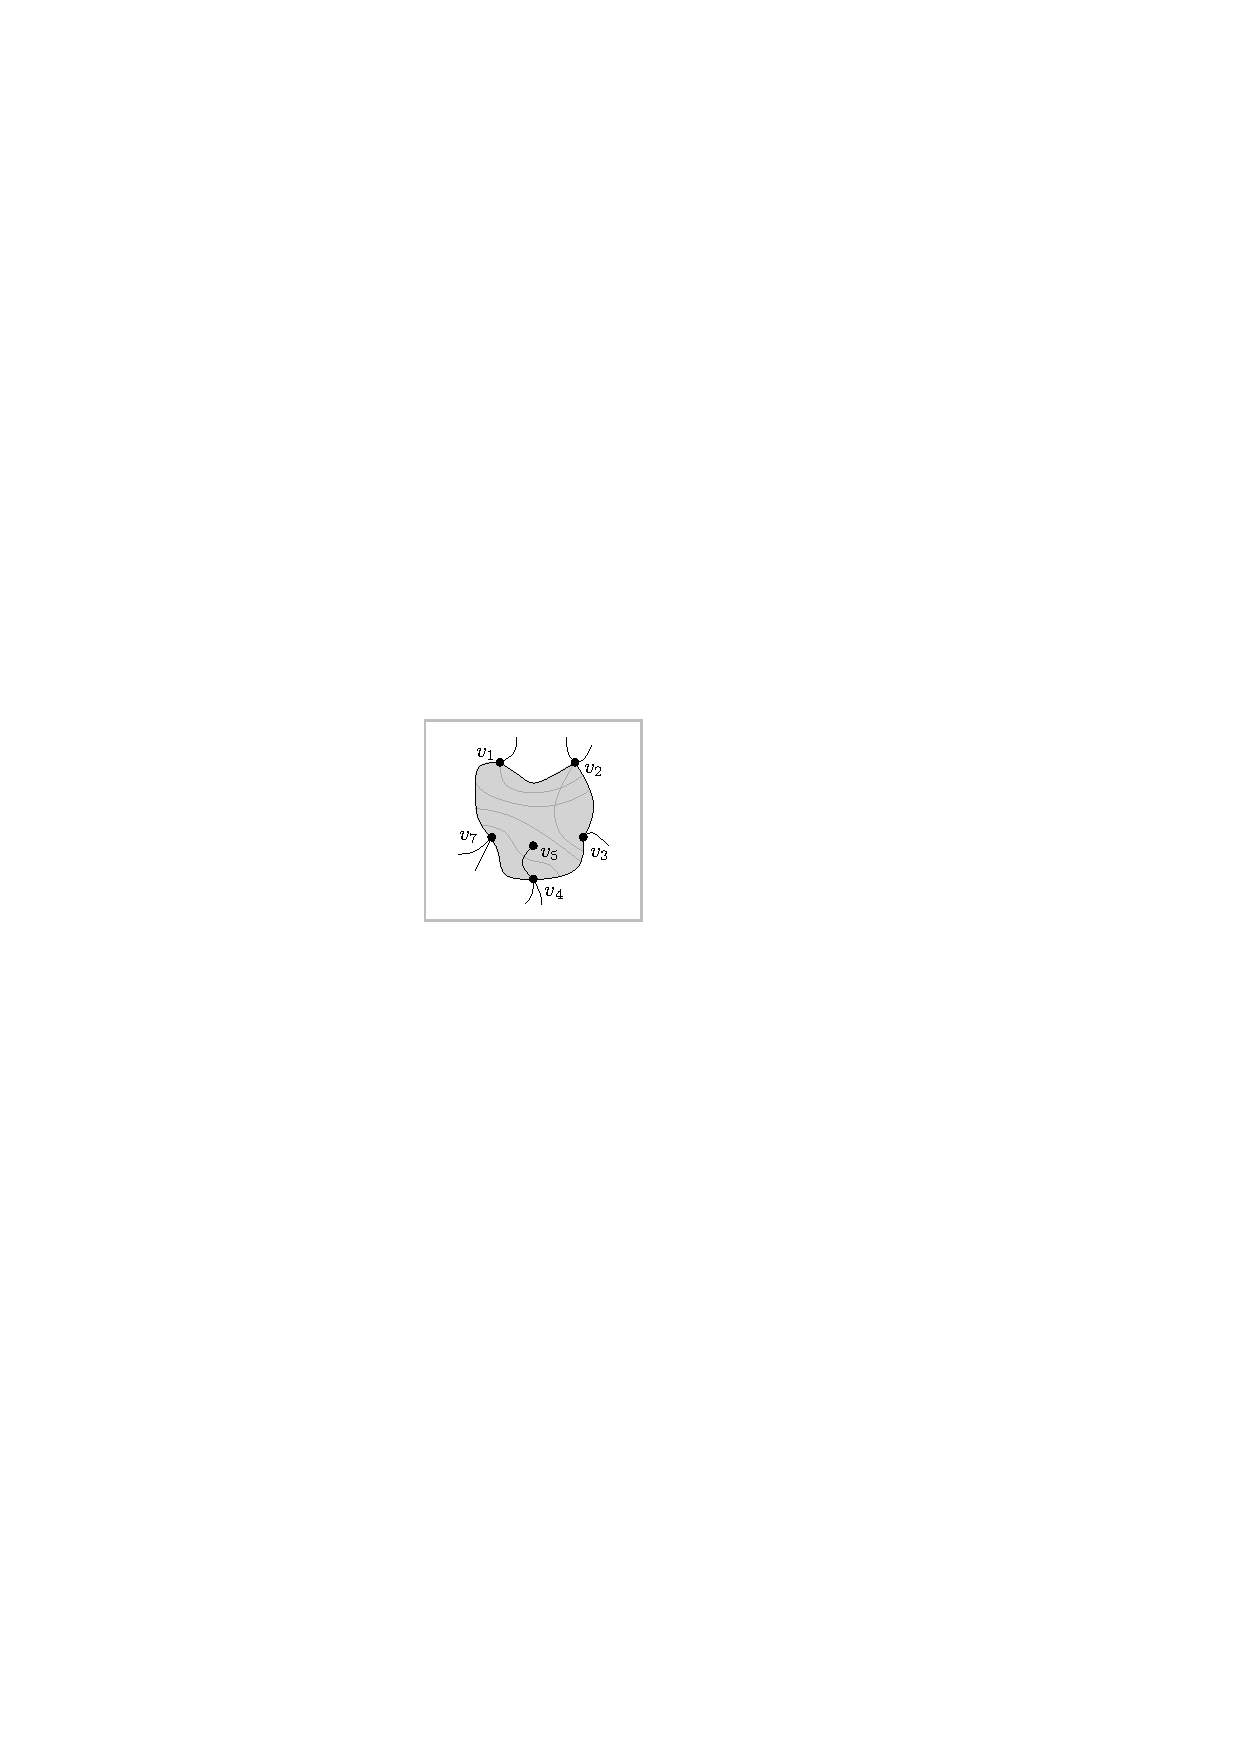
\includegraphics[width=\textwidth,page=1]{images/preliminaries}
        \subcaption{~}\label{fig:non_simple_face}
    \end{minipage}	
    \begin{minipage}[b]{.18\textwidth}
        \centering
        \includegraphics[width=\textwidth,page=2]{images/crossing_conf}
        \subcaption{~}\label{fig:crossing_twice_2}
    \end{minipage}
	\begin{minipage}[b]{.18\textwidth}
        \centering
        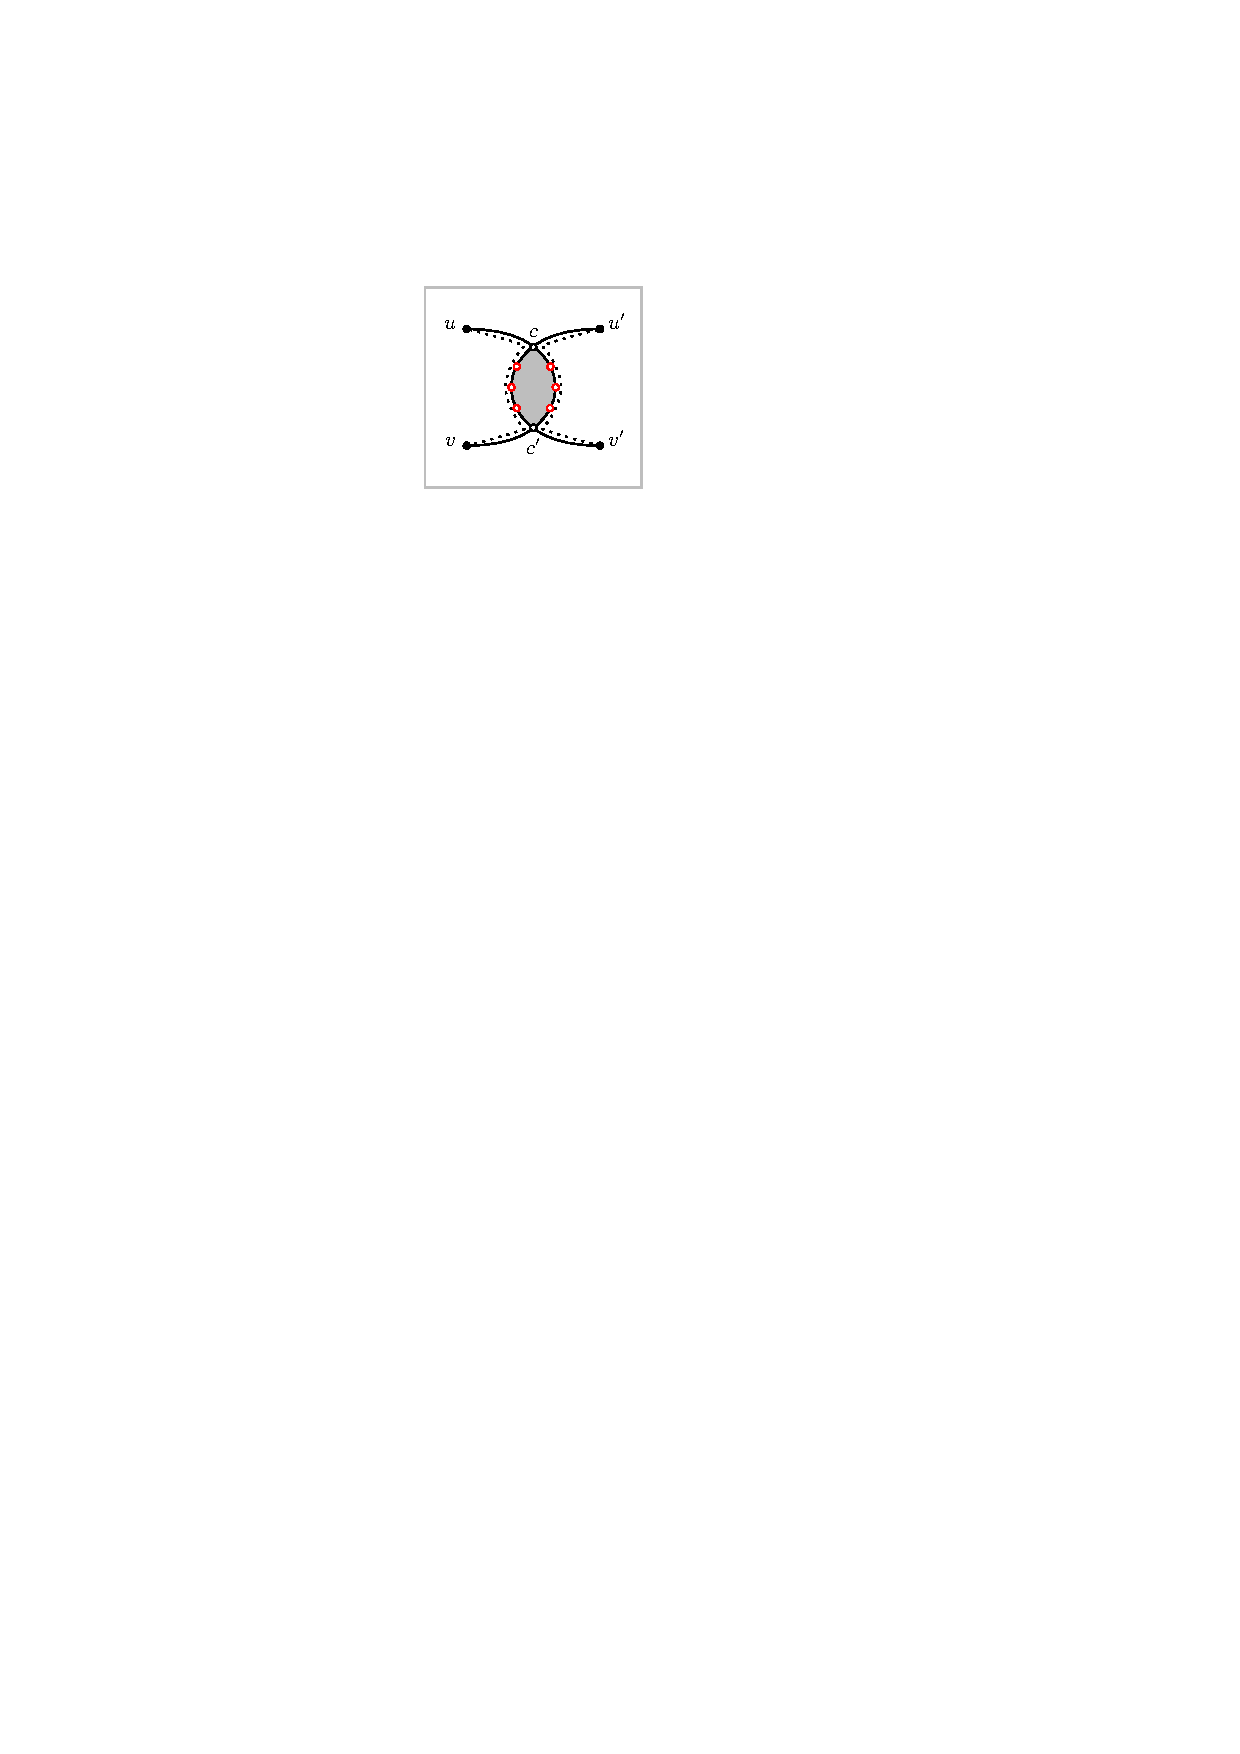
\includegraphics[width=\textwidth,page=1]{images/crossing_conf}
        \subcaption{~}\label{fig:crossing_twice}
    \end{minipage}
    \begin{minipage}[b]{.18\textwidth}
        \centering
        \includegraphics[width=\textwidth,page=3]{images/crossing_conf}
        \subcaption{~}\label{fig:crossing_adjacent}
    \end{minipage}	
    \begin{minipage}[b]{.18\textwidth}
        \centering
        \includegraphics[width=\textwidth,page=4]{images/crossing_conf}
        \subcaption{~}\label{fig:crossing_adjacent_2}
    \end{minipage}	
    \caption{%
    (a)~A non-simple face $\{v_1,\ldots,v_7\}$, where $v_6$ is identified with $v_4$.
    Different configurations used in 
    (b-c)~Lemma~\ref{lem:crossing_twice}, and 
    (d-e)~Lemma~\ref{lem:crossing_adjacent}.}
    \label{fig:2_planar_polygon_conf}
\end{figure} 

Drawing $\Gamma(G)$ is called \emph{$k$-planar} if every edge in $\Gamma(G)$ is crossed at most $k$ times. Accordingly, a graph is called \emph{$k$-planar} if it admits a $k$-planar drawing. An \emph{optimal $k$-planar} graph is a $k$-planar graph with the maximum number of edges (e.g., an optimal $1$-planar graph on $n$ vertices is a $1$-planar graph with exactly $4n-8$ edges). For an optimal $k$-planar graph $G$ on $n$ vertices, a $k$-planar drawing $\Gamma(G)$ of $G$ is called \emph{planar-maximal crossing-minimal} or simply PMCM-drawing if and only if $\Gamma(G)$ has the maximum number of true-planar edges among all $k$-planar drawings of $G$ and, subject to this restriction, $\Gamma(G)$ has also the minimum number of crossings.

\begin{lemma}
Let $\Gamma(G)$ be a PMCM-drawing of an optimal $k$-planar graph $G$ in which two edges $(u,v)$ and $(u',v')$ cross more that once. Let $c$ and $c'$ be two consecutive crossing points along $(u,v)$. Then, the closed region $R_{c,c'}$ that is defined by the edge segments of $(u,v)$ and $(u',v')$ between $c$ and $c'$ has at least one vertex in its interior and at least one vertex in its exterior.
\label{lem:crossing_twice}
\end{lemma}
\begin{proof}
We will prove that $R_{c,c'}$ has at least one vertex in its interior; the proof that $R_{c,c'}$ has at least one vertex in its exterior is analogous. For a proof by contradiction, assume that there exists a pair of edges which cross twice and $R_{c,c'}$ contains no vertices in its interior. Let $(u,v)$ and $(u',v')$ be such a pair with crossings $c$ and $c'$ which is \emph{minimal} in the sense that, if $(u,v)$ crosses twice an edge  $(u'',v'')$, then along $(u,v)$ the two crossings cannot be both between $c$ and $c'$; for an example see Figure~\ref{fig:crossing_twice_2}.

Let $nc(u,v)$ and $nc(u',v')$ be the number of crossings along $(u,v)$ and $(u',v')$ that are between $c$ and $c'$, respectively (red drawn in Figure~\ref{fig:crossing_twice}). First observe that by the 'minimality' criterion of $(u,v)$ and $(u',v')$ we have $nc(u,v) = nc(u',v')$. We redraw edges $(u,v)$ and $(u',v')$ by exchanging the middle segments between $c$ and $c'$ and eliminate both crossings $c$ and $c'$ without affecting the $k$-planarity of $G$; see the dotted-drawn edges of Figure~\ref{fig:crossing_twice}. Of course, this contradicts the crossing minimality of $\Gamma(G)$.
\end{proof}
 
\begin{lemma}
Let $\Gamma(G)$ be a PMCM-drawing of an optimal $k$-planar graph $G$ in which two edges $(u,v)$ and $(u,v')$ incident to a common vertex $u$ cross. Let $c$ be the first crossing point of $(u,v)$ with $(u,v')$ starting from $u$. Then, the closed region $R_{c}$ that is defined by the edge segments of $(u,v)$ and $(u,v')$ between $u$ and $c$ has at least one vertex in its interior and at least one vertex in its exterior.\todo{Simpler with minimality assumption ?} 
\label{lem:crossing_adjacent}
\end{lemma}
\begin{proof}
We will prove that $R_{c}$ has at least one vertex in its interior; the proof that $R_{c}$ has at least one vertex in its exterior is
analogous. For a proof by contradiction, assume that $R_{c}$ contains no vertices in its interior. Denote by $nc(u,v)$ and $nc(u,v')$ the number of crossings along $(u,v)$ and $(u,v')$ that are between $u$ and $c$, respectively (red drawn in Figure~\ref{fig:crossing_twice_2}). First assume that $nc(u,v) = nc(u,v')$. We will cope with the case where $nc(u,v) \neq nc(u,v')$ shortly. We proceed by eliminating crossing $c$ without affecting the $k$-planarity of $G$; see the dotted-drawn edges of Figure~\ref{fig:crossing_adjacent}. Of course, this contradicts the crossing minimality of $\Gamma(G)$. To complete the proof of this property, it remains to consider the case where $nc(u,v) \neq nc(u,v')$. Assume w.l.o.g.~that $nc(u,v) > nc(u,v')$. In this case, there is either one other edge of $u$, say $(u,v'')$ that crosses $(u,v)$ between $u$ and $c$, or there exists an edge $(u'',v'')$ that crosses at least twice edge $(u,v)$. By Lemma~\ref{lem:crossing_twice}, the latter case would imply that $R_{c}$ is not an empty region; a contradiction.  Hence, there exists at least one other edge, say $(u,v'')$, that crosses $(u,v)$ between $u$ and $c$, say at point $d$; refer to Figure~\ref{fig:crossing_adjacent_2}. Since the ``length'' between $u$ and $d$ is shorter than the length between $u$ and $c$, it follows that if we apply the analysis above on $(u,v)$ and $(u,v'')$, then there will be eventually a pair of crossing edges incident to $u$, say $e$ and $e'$ that have exactly the same number of crossings, that is, $nc(e) = nc(e')$. This pair of edges contradicts the crossing minimality of $\Gamma(G)$.   
\end{proof}

In several of our proofs we deploy a strategy according to which starting from an optimal $2$- or $3$-planar graph $G$, we modify $G$ and its drawing $\Gamma(G)$ by adding and removing elements (vertices or edges) without affecting $2$- or $3$-planarity, so that the number of edges in the derived graph $G'$ force $G$ to have fewer or more edges than required by optimality. Hence, $G$ was not optimal in first place. For the strategy to be deployed correctly, we have to assure that we do not introduce any homotopic parallel edges or self-loops, and that we do not deviate basic properties of the drawing (e.g., introduce an edge that crosses itself). The question that naturally arises is how to select and draw the newly inserted elements. The following definition introduces the notion of \pes, a collection of edges that our strategy can safely use.

A Jordan curve $[u,v]$ connecting vertices $u$ and $v$ of $G$ is called a \emph{\pe} in drawing $\Gamma(G)$ if and only if $[u,v]$ does not cross itself and is not a homotopic self-loop in $\Gamma(G)$, that is, either $u \neq v$ or $u=v$ and there is at least one vertex in the interior and the exterior of $[u,v]$. Note that $u$ and $v$ are not necessarily adjacent in $G$. However, since each topological edge $(u,v) \in E$ of $G$ is represented by a Jordan curve in $\Gamma(G)$, it follows that edge $(u,v)$ is by definition a \pe of $G$ (among other edges that can potentially exist).

Furthermore, we say that vertices $v_1,v_2,\dots,v_s$ define a \emph{\pp} in $\Gamma(G)$, if there exist \pes $[v_i,v_{i+1}]$, for $i=1,\dots, s-1$ and \pe $[v_1,v_s]$ of $\Gamma(G)$, which %
\begin{inparaenum}[(i)]
\item do not cross with each other and
\item define a region in $\Gamma(G)$ that has no vertices in its interior.
\end{inparaenum}

\begin{lemma}
Let $\Gamma(G)$ be a PMCM-drawing of a $k$-planar graph $G$. Let also $\mathcal{C}_s$ be a \pp of length $\nu$ in $\Gamma(G)$ and assume that $\kappa$ edges of $\Gamma(G)$ are drawn completely in the interior of $\mathcal{C}_s$, while $\lambda$ edges of $\Gamma(G)$ are crossing\footnote{Note that the boundary edges of $\mathcal{C}$ are not necessarily present in $\Gamma(G)$.} the boundary of $\mathcal{C}_s$. Also, assume that if one isolates $\mathcal{C}_s$ from $\Gamma(G)$, then $\mu$ non-homotopic edges can be drawn completely in the interior of $\mathcal{C}_s$ without deviating $k$-planarity. 
\begin{enumerate}[\emph{(}i\emph{)}]
\item \label{prp:nonoptim} If $\mu > \kappa + \lambda$, then $G$ is not optimal.
\item \label{prp:boundary} If $G$ is optimal and $\mu = \kappa + \lambda$, then all boundary edges of $\mathcal{C}_s$ exist\footnote{We say that a Jornan curve $[u,v]$ \emph{exists} in $\Gamma(G)$ if and only if $[u,v]$ is homotopic to an edge in $\Gamma(G)$.} in $\Gamma(G)$.
\end{enumerate}
\label{lem:exchange}
\end{lemma}
\begin{proof}
(\ref*{prp:nonoptim})~If we could replace the $\kappa + \lambda$ edges of $\Gamma(G)$ that are either drawn completely in the interior of $\mathcal{C}_s$ or cross the boundary of $\mathcal{C}_s$ with the $\mu$ ones that one can draw exclusively in the interior of $\mathcal{C}_s$, then the lemma would trivially follow. However, to do so we need to ensure that this operation introduces neither homotopic parallel edges nor homotopic self-loops. Since the edges that we introduce are \pes, it follows that no homotopic self-loops are introduced. We claim that homotopic paralled edges are not introduced either. In fact, if $e$ and $e'$ are two homotopic parallel edges, then both  must be drawn completely in the interior of $\mathcal{C}_s$, which implies that $e$ and $e'$ are both newly-introduced edges; a contradiction, since we introduce $\mu$ non-homotopic edges. (\ref*{prp:boundary})~In the exchanging scheme that we just described, except for the $\mu$ edges that one can draw exclusively in the interior of $\mathcal{C}_s$, one can also draw the boundary edges of $\mathcal{C}_s$ in $\Gamma(G)$, as long as they do not already exist in $\Gamma(G)$. Since $G$ is optimal, these edges must be present in $\Gamma(G)$ as well. 
\end{proof}



